% !TeX spellcheck = de_DE
\documentclass{uebung_cs}
\usepackage{algo123}
\uebung{2}{}{}
\blattname{Suchen und Sortieren (Woche 2)}

%%%%%%%%%%%%%%%%%%%%%%%%%%%%%%%%%%%%%%%%%%%%%%%%%%%%%%%%%%%%%%%%%%%%%%%%%%%%


\begin{document}

\textbf{Eigenständige Vorbereitung:}\\
Lies \emoji{book} CLRS Kapitel 2 und schau dir die \emoji{television} Videos der Woche an.
Beantworte dabei die folgenden Leitfragen:
\begin{enumerate}
	\item Wieso können wir sicher sein, dass binäre Suche immer das gesuchte Element findet, obwohl er sich nicht alle Elemente des Arrays anschaut? Wie viele Elemente schaut er sich an?
	\item An welchen Stellen in der Analyse von binärer Suche, insertion sort oder merge sort wird der kleine Satz von Gauß bzw.~die geometrische Reihe benutzt?
\end{enumerate}

\textbf{Zeichenlegende:}
\legende{}


%  \schriftlich
%  \bestehen
%  \mittel
%  \note
%  \spass

\begin{aufgabe}[Von Hand laufen lassen und Eigenschaften \bestehen]\label{tue-first}\mbox{}
	\begin{enumerate}
		\item (\warmup) Beschreibe den Ablauf von insertion sort, wenn die Eingabe ein Feld $A=[31,41,59,26,41,58]$ ist.
		\item (\warmup) Verändere den Pseudocode für insertion sort, um das Eingabefeld monoton fallend anstatt monoton wachsend zu ordnen.	
		\item Analysiere die Laufzeit von linearer Suche \emph{im mittleren Fall}: Wenn das gesuchte Element~$x$ zufällig und gleichwahrscheinlich irgendeines der Elemente von $A$ ist, wie viele Einträge von $A$ prüft lineare Suche dann, um $x$ zu finden?
		\item (\warmup) Beschreibe den Ablauf von merge sort auf dem Feld $A=[3,41,52,26,38,57,9,49]$.
		\item Überzeuge dich, dass insertion sort auch rekursiv wie folgt formuliert werden kann: um $A[0..n-1]$ zu sortieren, sortieren wir $A[0..n-2]$ rekursiv und fügen dann $A[n-1]$ in das sortierte Feld $A[0..n-2]$ ein. Stelle die Rekursionsgleichung für die Laufzeit dieses Algorithmus auf und löse sie.
		\item Ein Freund schlägt vor, dass du binäre Suche nutzen solltest, um den Einfügeschritt von insertion sort schneller zu machen. Funktioniert das, und welchen Effekt hat es auf die Laufzeit des Algorithmus?
	\end{enumerate}
\end{aufgabe}

\begin{aufgabe}[Duplikate und nahe Nachbarn \mittel]
	Sei $A[0..n-1]$ ein Feld von ganzen Zahlen.
	\begin{enumerate}
		\item (\warmup) Ein \emph{Duplikat} in $A$ ist ein Paar $(i,j)$ von unterschiedlichen Indizes mit $A[i]=A[j]$. Entwirf einen Algorithmus an, der in Zeit $O(n^2)$ findet, ob $A$ ein Duplikat hat.
		\item Entwirf einen Algorithmus an, der in Zeit $O(n\log n)$ findet, ob $A$ ein Duplikat hat. \emph{Hinweis:} Nutze merge sort.
		\item Ein \emph{nächstes Paar} in $A$ ist ein Paar $(i,j)$ mit $i\ne j$, sodass der Abstand $|A[i]-A[j]|$ minimal ist unter allen Paaren von Einträgen.
		Entwerfe einen Algorithmus, der den Abstand eines nächsten Paars in Zeit $O(n\log n)$ findet.
	\end{enumerate}
\end{aufgabe}

\begin{aufgabe}[Korrektheit von Merge Sort \mittel]
	Beweise, dass Merge Sort alle gegebenen Felder korrekt sortiert. Hierbei darfst du annehmen, dass die Verflechtungsoperation \textsc{Merge} auf sortierten Feldern korrekt arbeitet.
	\emph{Hinweis: benutze vollständige Induktion.}
\end{aufgabe}

\begin{aufgabe}[2-Summe und 3-Summe]
	Sei $A[0..n-1]$ ein Feld von ganzen Zahlen (positive und negative Zahlen sind erlaubt).
	Das Feld $A$ hat eine \emph{2-Summe}, wenn es zwei Einträge $i$ und~$j$ gibt mit $A[i]+A[j]=0$.
	Analog hat $A$ eine \emph{3-Summe}, wenn es drei Einträge $i$, $j$, und $k$ gibt, sodass $A[i]+A[j]+A[k]=0$.
	\begin{enumerate}
		\item \bestehen %(\warmup)
    Gib einen einfachen Algorithmus an, der in Zeit $O(n^2)$ feststellt, ob $A$ eine 2-Summe hat.
		\item \mittel Gib einen Algorithmus an, der in Zeit $O(n\log n)$ feststellt, ob $A$ eine 2-Summe hat. \emph{Hinweis: binäre Suche.}
		\item \bestehen %(\warmup)
    Gib einen Algorithmus an, der in Zeit $O(n^3)$ feststellt, ob $A$ eine 3-Summe hat.
		\item \mittel Gib einen Algorithmus an, der in Zeit $O(n^2\log n)$ feststellt, ob $A$ eine 3-Summe hat. \emph{Hinweis: binäre Suche.}
		\item \note (\veryhard) Gib einen Algorithmus an, der in Zeit $O(n^2)$ feststellt, ob $A$ eine 3-Summe hat.
	\end{enumerate}
\end{aufgabe}

\begin{aufgabe}[Auswahl, Partition, und Quick Sort]
Sei $A[0..n-1]$ ein Feld von unterschiedlichen ganzen Zahlen.
Der Eintrag von \emph{Rang $k$} in $A$ ist die $k$t kleinste Zahl unter den Zahlen in $A$.
Der \emph{Median} von $A$ ist die Zahl von Rang $\lceil(n/2)\rceil$.
\begin{enumerate}
	\item \mittel Gib einen Algorithmus mit Laufzeit $O(n\log n)$ an, der $A$ und $k$ als Eingabe nimmt und die Zahl in $A$ ausgibt, die Rang $k$ hat.
\end{enumerate}
Eine \emph{Partition} von $A$ ist eine Aufteilung in Felder $A_{\text{low}}$ und $A_{\text{high}}$, sodass $A_{\text{low}}$ alle Zahlen von $A$ enthält, die kleiner oder gleich dem Median von $A$ sind, und $A_{\text{high}}$ alle Zahlen von $A$ enthält, die größer sind als der Median von $A$.
Es gibt einen Linearzeitalgorithmus, der den Median eines Feldes findet; diesen Algorithmus darfst du im Folgenden einfach annehmen.
\begin{enumerate}[resume]
	\item \bestehen Gib einen Algorithmus an, der eine Partition von $A$ in Zeit $O(n)$ ausrechnet.
	\item \note %(\hard)
  Gib einen Algorithmus an, der $A$ in Zeit $O(n\log n)$ sortiert, indem er rekursiv partitioniert.
	\item \note (\veryhard) Gib einen Algorithmus mit Laufzeit $O(n)$ an, der $A$ und $k$ als Eingabe nimmt und die Zahl in $A$ ausgibt, die Rang $k$ hat.
\end{enumerate}
\end{aufgabe}


\begin{aufgabe}[$k$-Merge Sort]
	Professorin M.\ Erge stellt ihren neuen Algorithmus, 3-Merge Sort, vor.
	3-Merge Sort funktioniert genau wie das uns bekannte Merge Sort, nur wird rekursiv in drei Teile anstatt zwei aufgeteilt, die daraufhin sortiert und wieder verflochten werden.
	Löse die folgenden Teilaufgaben.
	\begin{enumerate}
		\item \mittel Zeige, dass sich drei sortierte Felder in asymptotischer Linearzeit verflechten lassen.
		\item \bestehen Führe eine Laufzeitanalyse für 3-Merge Sort durch. Stelle hierzu die Rekursionsgleichung für die Laufzeit $T(n)$ auf und löse diese.
		\item \note %(\hard)
    Verallgemeinere den Algorithmus und die Analyse von 3-Merge Sort zu $k$-Merge Sort für $k>3$.\\
		Hat Prof.\ M.\ Erge den Durchbruch geschafft?
		Stellt $k$-Merge Sort eine Verbesserung gegenüber dem klassischen 2-Merge Sort dar?
	\end{enumerate}
\end{aufgabe}

\newpage
\begin{aufgabe}[Kreuzende Linien \schriftlich]
  Gegeben seien zwei Sequenzen von Punkten in der $xy$-Ebene, nämlich $p_1,\dots,p_n$ auf der Linie $y=0$ und $q_1,\dots,q_n$ auf der Linie $y=1$.
	Erzeuge nun $n$ Strecken, indem jeder Punkt $p_i$ mit $q_i$ verbunden wird.
	Beschreibe und analysiere einen \emph{divide-and-conquer} Algorithmus, der in Zeit $O(n \log n)$ ausrechnet, wie viele Paare von Strecken sich schneiden.

	Zum Beispiel gibt es unter den folgenden 7 Strecken genau 8 Paare von Strecken, die sich schneiden:
	\begin{center}
	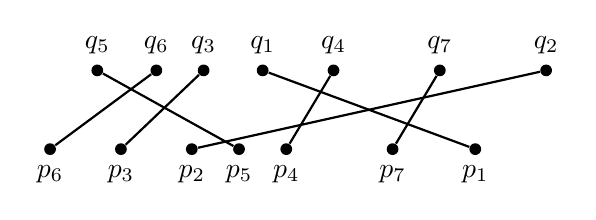
\begin{tikzpicture}[xscale=1.5]
		\node[fill,circle,inner sep=1.5pt,label=below:{$p_1$}] (p1) at (4,0) {};
		\node[fill,circle,inner sep=1.5pt,label=below:{$p_2$}] (p2) at (1.6,0) {};
		\node[fill,circle,inner sep=1.5pt,label=below:{$p_3$}] (p3) at (1,0) {};
		\node[fill,circle,inner sep=1.5pt,label=below:{$p_4$}] (p4) at (2.4,0) {};
		\node[fill,circle,inner sep=1.5pt,label=below:{$p_5$}] (p5) at (2,0) {};
		\node[fill,circle,inner sep=1.5pt,label=below:{$p_6$}] (p6) at (0.4,0) {};
		\node[fill,circle,inner sep=1.5pt,label=below:{$p_7$}] (p7) at (3.3,0) {};
		\node[fill,circle,inner sep=1.5pt,label=above:{$q_1$}] (q1) at (2.2,1) {};
		\node[fill,circle,inner sep=1.5pt,label=above:{$q_3$}] (q3) at (1.7,1) {};
		\node[fill,circle,inner sep=1.5pt,label=above:{$q_2$}] (q2) at (4.6,1) {};
		\node[fill,circle,inner sep=1.5pt,label=above:{$q_4$}] (q4) at (2.8,1) {};
		\node[fill,circle,inner sep=1.5pt,label=above:{$q_5$}] (q5) at (0.8,1) {};
		\node[fill,circle,inner sep=1.5pt,label=above:{$q_6$}] (q6) at (1.3,1) {};
		\node[fill,circle,inner sep=1.5pt,label=above:{$q_7$}] (q7) at (3.7,1) {};
		\foreach\i in {1,...,7} {
			\draw[thick] (p\i)--(q\i);
		}
	\end{tikzpicture}
	\end{center}
	
	Die Eingabe soll gegeben sein als zwei Felder $p[1..n]$ und $q[1..n]$ von ganzen Zahlen, sodass $p[i]$ die $x$-Koordinate von $p_i$ beschreibt und $q[j]$ die $x$-Koordinate von $q_j$. Sie dürfen annehmen, dass alle $x$-Koordinaten verschieden sind. 
\end{aufgabe}

\input{allgemeine-kriterien-23.inc}
\end{document}
